% !TEX root = saveliev_physics_general_course_1.tex
%!TEX TS-program = pdflatex
%!TEX encoding = UTF-8 Unicode


\chapter{RELATIVISTIC MECHANICS}\label{chap:8}

\section{The Special Theory of Relativity}\label{sec:8_1}

It was noted in Sec.~\ref{sec:2_1} that Newtonian mechanics holds only for bodies travelling with speeds that are much lower than the speed of light in a vacuum (this speed is denoted by the symbol $c$). To describe motion at speeds comparable with $c$, Albert Einstein advanced relativistic mechanics, \ie, mechanics taking the requirements of the special theory of relativity into account.

The special theory of relativity presented by Einstein in 1905 is a physical theory of space and time\footnote{In 1915, Einstein presented the fundamentals of the general theory of relativity, which is the theory of gravitation.}. The foundation of this theory is formed by two postulates called \textbf{Einstein's principle of relativity} and the \textbf{principle of constancy of the speed of light}. 

Einstein's principle of relativity is an extension of Galileo' mechanical principle (see Sec.~\ref{sec:2_7} to all physical phenomena without any exception. According to this principle, \textit{all laws of nature are the same in all inertial reference frames}. The unchanged form of an equation when the coordinates and time of one reference frame are replaced in it with the coordinates and time of another frame is called the \textbf{invariance} of the equation. The principle of relativity can therefore be formulated as follows: \textit{the equations expressing the laws of nature are invariant with respect to transformations of coordinates and time from one inertial reference frame to another}.

The principle of constancy of the \textit{speed of light states that the speed of light in a vacuum is the same in all inertial reference frames and does not depend on the motion of the sources and receivers of light}.\footnote{The experiment performed by A. Michelson and E. Morley confirming the validity of this principle will be described in the second volume of our course.}

A number of important conclusions relating to the properties of space and time follow from the above postulates. Space and time were considered independently of each other in Newtonian mechanics. Newton considered that absolute space and absolute time exist. He defined absolute space as a container of articles that always remains the same and stationary and that bas no relation to anything external. Newton wrote about time that absolute, true, or mathematical time flows uniformly without any relation to anything external by itself and owing to its internal nature. Accordingly, it was considered absolutely obvious that two events occurring simultaneously in one reference frame will also be simultaneous in all other reference frames. It is easy to see, however, that the latter statement contradicts the principle of the constancy of the speed of light.

Let us take two bodies K and K$'$ forming inertial reference frames together with their corresponding clocks. Assume that body K$'$ moves relative to body K with the velocity $\vec{v}_0$ directed along the straight line passing through the centres of the bodies (\fig{8_1}). Let us put two bodies M and N on this line. The bodies are at equal distances from body K$'$ and are rigidly joined to it. These bodies move relative to body K with the velocity $\vec{v}_0$, and are at rest relative to body K$'$. Let us consider the same process in both frames, namely, the emission of a light signal from the centre of body K$'$ and its reaching bodies M and N. The speed of light in all directions is the same and equals $c$. Hence, in the reference frame K$'$, the signal will reach bodies M and N at the same moment $t'$.

\begin{figure}[t]
	\begin{center}
		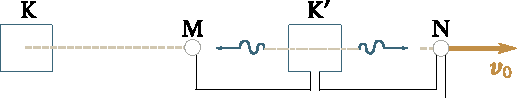
\includegraphics[scale=0.95]{figures/cap_08/fig_8_1.pdf}
		\caption[]{}
		\label{fig:8_1}
	\end{center}
	\vspace{-0.8cm}
\end{figure}

In the reference frame K, light also propagates in all directions with the speed $c$. In this frame, M moves toward the light signal. Body N moves in the same direction as the signal. Consequently, the signal reaches M before it reaches N, and therefore $t_{\text{M}}<t_{\text{N}}$. Thus, the events that were simultaneous in the frame K$'$ will not be simultaneous in the frame K. Hence, it follows that time flows differently in different reference frames.

To describe an event in a reference frame, we must indicate the place and the moment at which it occurs. This task can be coped with if we set up equally spaced coordinate marks in space and put a clock at each mark that will permit us to determine the moment at which the event occurs at the given place. The coordinate marks can be made by transferring a unit scale. Any system performing a periodically repeating process can be used as a clock. To compare the moments at which two events occur at different points of space, we must see that the clocks at these points are synchronized.

It would seem possible to synchronize the clocks by first placing them next to one another, and then, after comparing their readings, by transferring them to the corresponding points of space. Such a method must be rejected, however, because we do not know how the transfer of the clocks from one place to another will affect their running. We must therefore first put the clocks at their relevant places and only then compare their readings. This can be done by sending a light signal from one clock to the others\footnote{The checking of clocks according to radio signals is in essence such synchronization.}. Assume that a light signal is sent from point A at the moment $t_1$ (according to the clock at A). The signal is reflected from a mirror at point B and returns to A at the moment $t_2$. The clock at B should be considered synchronized with the one at A if at the moment when the signal reaches it the clock at B shows the time $t$ equal to $(t_1+t_2)/2$. This procedure must be performed for all the clocks arranged at the different points of the frame K. The events at A and B will be considered simultaneous in the frame K if the readings of the clocks at A and B corresponding to them coincide.

All the clocks in the frame K$'$ and in any other inertial reference frame are synchronized in a similar way. The speed of the light signal used for synchronization is the same in all the inertial reference frames. This explains why it is a light signal that is chosen as the signal for clock synchronization. The speed of light was found to be the limit. No signal, no action of one body on another can propagate with a speed exceeding that of light in a vacuum. This is the reason for light having the same speed in a vacuum in all reference frames. According to the principle of relativity, the laws of nature in all inertial frames must be identical. The circumstance that the speed of a signal cannot exceed a limiting value is also a law of nature. Hence, the value of the limiting speed must be the same in all reference frames.

The constancy of the speed of light results in space and time being mutually related, forming a single space-time. This relation can be depicted especially clearly with the aid of an imaginary four-dimensional space along three axes of which the space coordinates $x, y, z$ are laid off, and along the fourth axis the time $t$, more exactly the time coordinate $ct$ proportional to $t$ and having the same dimension as the space coordinates.

An event (for instance, the decay of a particle) is characterized by the place where it occurred (by the coordinates $x, y, z$) and by the time $t$ when it occurred. Thus, a point with the coordinates $x, y, z, ct$ corresponds to an event in our imaginary four-dimensional space. This point is called the \textbf{world point}. A line called the \textbf{world line} corresponds to any particle (even a stationary one) in four-dimensional space (for a particle at rest it has the form of a straight line parallel to the $ct$-axis).

Thus, space and time are parts of a single whole. But time differs qualitatively from space. This manifests itself in that our imaginary four-dimensional space differs in its properties from the conventional three-dimensional space. The latter has Euclidean metric. This signifies that the square of the distance $\Delta l$ between two points equals the sum of the squares of the coordinate differences:
\begin{equation*}
	\Delta l^2 = \Delta x^2 + \Delta y^2 + \Delta z^2.
\end{equation*}

The square of the ``distance'' between two world points (this distance is called an \textbf{interval} and is designated by the symbol $\Delta s$) is determined by the equation
\begin{equation}\label{eq:8_1}
	\Delta s^2 = c^2\Delta t^2 - \Delta x^2 - \Delta y^2 - \Delta z^2
\end{equation}

\noindent
(the properties of an interval are treated in Sec.~\ref{sec:8_4}).

Spaces for which the square of the distance is determined by a formula such as~\eqref{eq:8_1} are called \textbf{pseudo-Euclidean}. The qualitative distinction between time and space manifests itself in that the square of the time coordinate and the squares of the space coordinates enter \eqn{8_1} with different signs.

A distinctive part in the special theory of relativity is played by quantities that are \textbf{invariant} with respect to the transformations of the coordinates and time from one inertial reference frame to another (in other words, quantities having the same numerical value in all inertial reference frames). We know one such quantity, namely, the speed of light in a vacuum. We shall show in Sec.~\ref{sec:8_4} that the interval defined by \eqn{8_1} is also an invariant.

A distinctive part is also played by equations and relations that are invariant with respect to the transformations indicated above (\ie, having the same form in all inertial reference frames). For example, the relativistic expressions for the momentum and energy are determined so that the laws of conservation of these quantities are not violated when transferring to another inertial reference frame. We shall acquaint ourselves with a number of invariant quantities and relations in our further treatment.

\section{Lorentz Transformations}\label{sec:8_2}

Let us consider two inertial reference frames K and K$'$ (\fig{8_2}). Assume that the frame K$'$ moves relative to the frame K with the velocity $\vec{v}_0$\footnote{We remind our reader that the name inertial is used to designate a reference frame relative to which a free particle moves without acceleration (see Sec.~\ref{sec:2_2}). In Sec.~\ref{sec:2_7}, we showed on the basis of the Galilean transformation that the frame K$'$ moving relative to the inertial frame K with the constant velocity	$\vec{v}_0$ is also inertial, in turn. In relativistic mechanics, the Galilean transformations have to be replaced with other ones that agree with the principle of the constancy of the speed of light. It is clear, however, that no matter what the law of transformation is when passing from the frame K to the frame K$'$ moving relative to it with the constant velocity $\vec{v}_0$ , if the velocity $\vec{v}$ of a particle in the frame K is constant, then its velocity $\vec{v}'$ in the frame K$'$ will also be constant. Consequently, in relativistic mechanics too, the frame K$'$ moving with a constant velocity $\vec{v}_0$ relative to the inertial frame K will also be inertial.}. Let us direct the axes $x$ and $x'$ along the vector $\vec{v}_0$, and assume that the axes $y$ and $z$ are parallel to the axes $y'$ and $z'$, respectively.

\begin{figure}[t]
	\begin{center}
		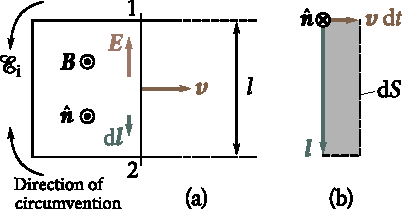
\includegraphics[scale=0.95]{figures/cap_08/fig_8_2.pdf}
		\caption[]{}
		\label{fig:8_2}
	\end{center}
	\vspace{-0.8cm}
\end{figure}

Owing to the principle of relativity, the frames K and K$'$ have absolutely equal rights. Their only formal distinction is that the $x$-coordinate of origin $0'$ of the frame K$'$ measured in the frame K changes according to the law
\begin{equation}\label{eq:8_2}
	x_{0'} = v_0 t
\end{equation}

\noindent
whereas the $x'$-coordinate of origin $0$ of the frame K measured in the frame K$'$ changes according to the law
\begin{equation}\label{eq:8_3}
	x'_0 = - v_0 t'.
\end{equation}

\noindent
This distinction is due to the fact that we have chosen identical directions of the axes $x$ and $x'$, but the frames K and K$'$ move in opposite directions relative to each other. Hence, the projection of the relative velocity of the frame K onto the $x$-axis is $\vec{v}_0$, and that of the frame K$'$ onto the $x'$-axis is $-\vec{v}_0$.

In non-relativistic mechanics, we used the Galilean transformation~\eqref{eq:2_9} to pass over from the coordinates and time of one inertial reference frame to the coordinates and time of another inertial frame. The rule of velocity addition $\vec{v}=\vec{v}'+\vec{v}_0$ [see \eqn{2_21}] follows from these transformations. This rule contradicts the principle of constancy of the speed of light. Indeed, if in the frame K$'$ a light signal propagates in the direction of the vector $\vec{v}_0$ with the velocity $c$, then according to \eqn{2_21} in the frame K the velocity of the signal will be $c+v_0$, \ie, it will exceed $c$. Hence, it follows that the Galilean transformations must be replaced with other formulas. It is not difficult to find the latter.

In the most general form, the transformations of the coordinates and time from the frame K$'$ to the frame K are as follows:
\begin{equation}\label{eq:8_4}
	\begin{cases}
		&\!\!\!\! x = f_1(x',y',z',t'),\quad y = f_2(x',y',z',t'),\\
		&\!\!\!\! z = f_3(x',y',z',t'),\quad t = f_4(x',y',z',t').
	\end{cases}
\end{equation}

\noindent
It follows from the uniformity of time and space that Eqs.~\eqref{eq:8_4} should be linear, \ie, have the form
\begin{equation}\label{eq:8_5}
	x = \alpha_1 x' + \alpha_2 y' + \alpha_3 z' + \alpha_4 t' + \alpha_5
\end{equation}

\noindent
and so on, where $\alpha_1, \alpha_2, \ldots$ are constants. Accordingly
\begin{equation}\label{eq:8_6}
	\deriv{x} = \alpha_1\,\deriv{x'} + \alpha_2\,\deriv{y'} + \alpha_3\,\deriv{z'} + \alpha_4\,\deriv{t'}
\end{equation}

\noindent
and so on.

Indeed, according to Eqs.~\eqref{eq:8_4}
\begin{align}
	\deriv{x} &= \diffpartial{f_1}{x'}\deriv{x'} + \diffpartial{f_2}{y'}\deriv{y'} + \diffpartial{f_3}{z'}\deriv{z'} + \diffpartial{f_4}{t'}\deriv{t'}\label{eq:8_7}\\
	&\vdots\quad\quad\vdots\quad\quad\vdots\quad\quad\vdots\quad\quad\vdots\quad\quad\vdots\quad\quad\vdots\nonumber
\end{align}

\noindent
If we take the arbitrarily chosen values $\deriv{x'}, \deriv{y'}, \deriv{z'}, \deriv{t'}$ for the point $x_1', y_1', z_1', t_1'$, then upon introducing into Eqs.~\eqref{eq:8_7} the values of the derivatives at the given point, we get a certain value $\deriv{x_1}$ for $\deriv{x}$. Owing to the uniformity of space and time, however, for any other point $x_2', y_2', z_2', t_2'$ at the same values $\deriv{x'}, \deriv{y'}, \deriv{z'}, \deriv{t'}$ we should get the same value for $\deriv{x}$ as for the first point, \ie, we should have $\deriv{x_2}=\deriv{x_1}$. The same should hold for $\deriv{y}, \deriv{z}$, and $\deriv{t}$. Since $\deriv{x'}, \deriv{y'}, \deriv{z'}, \deriv{t'}$ were chosen absolutely arbitrarily, this requirement can be observed only if the derivatives of $\diffinpartial{f_1}{x'}$, etc. do not depend on the coordinates, \ie, are constants. Hence follows \eqn{8_6}, and then also \eqn{8_5}.

With the choice of the coordinate axes shown in \fig{8_2}, the plane $y=0$ coincides with the plane $y'=0$ and the plane $z=0$ with the plane $z'=0$. It thus follows that, for example, the coordinates $y$ and $y'$ must become equal to zero simultaneously regardless of the values of the other coordinates and time. Therefore, $y$ and $y'$ can be related only by expressions of the kind
\begin{equation*}
	y = \varepsilon y'
\end{equation*}

\noindent
where $\varepsilon$ is a constant. Owing to the frames K and K$'$ having equal rights, the reverse relation must hold, \ie,
\begin{equation*}
	y' = \varepsilon y
\end{equation*}

\noindent
with the same value of the constant $\varepsilon$ as in the first case. Multiplication of these two equations yields $\varepsilon^2 = 1$, whence $\varepsilon=\pm 1$. The plus sign corresponds to the axes $y$ and $y'$ having the same directions, and the minus sign to their having opposite directions. Giving the axes the same direction, we get
\begin{equation}\label{eq:8_8}
	y = y'.
\end{equation}

\noindent
Similar reasoning yields
\begin{equation}\label{eq:8_9}
	z = z'.
\end{equation}

Now let us turn to finding the transformations for $x$ and $t$. It can be seen from Eqs.~\eqref{eq:8_8} and~\eqref{eq:8_9} that the values of $y$ and $z$ do not depend on $x'$ and $t'$. Hence, the values of $x'$ and $t'$ cannot depend on $y$ and $z$, correspondingly, the values of $x$ and $t$ cannot depend on $y'$ and $z'$. Thus, $x$ and $t$ can be linear functions of only $x'$ and $t'$.

The origin of coordinates $0$ of the frame K has the coordinate $x=0$ in the frame K and $x'=-v_0t'$ in the frame K$'$ [see \eqn{8_3}]. Consequently, the expression $(x'+v_0t')$ must vanish simultaneously with the coordinate $x$. For this to occur, the linear transformation should have the form
\begin{equation}\label{eq:8_10}
	x = \gamma (x' + v_0 t')
\end{equation}

\noindent
where $\gamma$ is a constant.

Similarly, the origin of coordinates $0'$ of the frame K$'$ has the coordinate $x'=0$ in the frame K$'$ and $x=v_0t$ in the frame K [see \eqn{8_2}]. Hence,
\begin{equation}\label{eq:8_11}
	x' = \gamma (x - v_0 t)
\end{equation}

\noindent
It follows from the frames K and K$'$ having equal rights that the constant of proportionality in both cases should be the same.

We shall use the principle of constancy of the speed of light to find the constant $y$. Let us begin to count the time in both frames from the moment when their origins of coordinates coincide. Assume that at the moment $t=t'=0$ a light signal is sent in the direction of the axes $x$ and $x'$ that causes a flash of light to appear on a screen at a point with the coordinate $x$ in the frame K and with the coordinate $x'$ in the frame K$'$. This event (flash) is described by the coordinate $x$ and the moment $t$ in the frame K, and by the coordinate $x'$ and the moment $t'$ in the frame K$'$, and
\begin{equation*}
	x = ct,\quad x' = ct'.
\end{equation*}

\noindent
Using these values of $x$ and $x'$ in Eqs.~\eqref{eq:8_10} and~\eqref{eq:8_11}, we get
\begin{align*}
	ct  &= \gamma (ct' + v_0 t') = \gamma (c + v_0)t',\\
	ct' &= \gamma (ct - v_0 t) = \gamma (c - v_0)t.
\end{align*}

Multiplication of these two equations yields
\begin{equation}\label{eq:8_12}
	\gamma = \frac{1}{\left[1 - \left(v_0^2/c^2\right)\right]^{1/2}}.
\end{equation}

\noindent
Introduction of this value into \eqn{8_10} gives
\begin{equation}\label{eq:8_13}
	x = \frac{x + v_0 t'}{\left[1 - \left(v_0^2/c^2\right)\right]^{1/2}}.
\end{equation}

Equation~\eqref{eq:8_13} allows us to find the value of $x$ according to known values of $x'$ and $t'$. To obtain an equation allowing us to find the value of $t$ according to the known values of $x'$ and $t'$, let us delete the coordinate $x$ from Eqs.~\eqref{eq:8_10} and~\eqref{eq:8_11} and solve the resulting expression relative to $t$. We obtain
\begin{equation*}
	t = \gamma \left[t' + \frac{x'}{v_0}\left(1 - \frac{1}{\gamma^2}\right)\right].
\end{equation*}

\noindent
Substituting for $\gamma$ its value from \eqn{8_12}, we have
\begin{equation}\label{eq:8_14}
	t = \frac{t' + (v_0/c^2) x'}{\left[1 - \left(v_0^2/c^2\right)\right]^{1/2}}.
\end{equation}

The combination of Eqs.~\eqref{eq:8_8}, \eqref{eq:8_9}, \eqref{eq:8_13}, and~\eqref{eq:8_14} is called \textbf{Lorentz transformations}. If we use the generally adopted symbol
\begin{equation}\label{eq:8_15}
	\beta = \frac{v_0}{c}
\end{equation}

\noindent
then the Lorentz transformations acquire the form
\begin{equation}\label{eq:8_16}
	x = \frac{x + \beta ct'}{\left(1 - \beta^2\right)^{1/2}},\quad y = y',\quad z = z',\quad t = \frac{t' + (\beta/c) x'}{\left(1 - \beta^2\right)^{1/2}}.
\end{equation}

Equations~\eqref{eq:8_16} allow us to pass over from coordinates and time measured in the frame K$'$ to those measured in the frame K (in short, to pass over from the frame K$'$ to the frame K). If we solve Eqs.~\eqref{eq:8_16} relative to the primed quantities, we get the equations for transformation from the frame K to K$'$:
\begin{equation}\label{eq:8_17}
	x' = \frac{x - \beta ct}{\left(1 - \beta^2\right)^{1/2}},\quad y' = y,\quad z' = z,\quad t' = \frac{t - (\beta/c) x}{\left(1 - \beta^2\right)^{1/2}}.
\end{equation}

As should be expected with a view to the equal rights of the frames K and K$'$, Eqs.~\eqref{eq:8_17} differ from their counterparts~\eqref{eq:8_16} only in the sign of $\beta$, \ie, of $v_0$.

It is easy to understand that when $v_0\ll c$ (\ie, $\beta\ll 1$), the Lorentz transformations become the same as the Galilean ones [see Eqs.~\eqref{eq:2_19}]. The latter thus retain their importance for speeds that are small in comparison with the speed of light in a vacuum.

When $v_0>c$, Eqs.~\eqref{eq:8_16} and~\eqref{eq:8_17} for $x$, $t$, $x'$, and $t'$ become imaginary. This agrees with the fact that motion at a speed exceeding that of light in a vacuum is impossible. It is impossible even to use a reference frame moving with the speed $c$ because when $v_0=c$, we get zero in the denominators of the equations for $x$ and $t$.

The Lorentz transformations have an especially simple and symmetrical form if we write them for $x$ and ($ct$) instead of for $x$ and $t$, \ie, for quantities of the same dimension. In this case, Eqs.~\eqref{eq:8_16} have the form
\begin{equation}\label{eq:8_18}
	x = \frac{x' + \beta (ct)'}{\left(1 - \beta^2\right)^{1/2}},\quad y = y',\quad z = z',\quad t = \frac{(ct)' + \beta x'}{\left(1 - \beta^2\right)^{1/2}}.
\end{equation}

It is simple to memorize Eqs.~\eqref{eq:8_18} by bearing in mind that the first of them differs from the ``obvious'' equation $x=x'+v_0t'$ in containing in its denominator the expression $\left(1 - \beta^2\right)^{1/2}$ characteristic of relativistic formulas. The last equation is obtained from the first one if we change the places of $x'$ and $ct'$.

\section{Corollaries of the Lorentz Transformations}\label{sec:8_3}

A number of corollaries follow from the Lorentz transformations that are unusual from the viewpoint of Newtonian mechanics.

\textbf{Simultaneity of Events in Different Reference Frames.} Assume that two events occur simultaneously in the frame K at points with the coordinates $x_1$ and $x_2$ and at the moment $t_1=t_2=b$. According to the last of the equations~\eqref{eq:8_17}, the moments
\begin{equation*}
	t_1' = \frac{b - (\beta/c) x_1}{\left(1 - \beta^2\right)^{1/2}},\quad t_2' = \frac{b - (\beta/c) x_2}{\left(1 - \beta^2\right)^{1/2}}
\end{equation*}

\noindent
will correspond to these events in the frame K$'$. Examination of these equations shows that if the events occur at different points of space ($x_1\neq x_2$) in the frame K, then they will not be simultaneous in the frame K$'$ ($t_1'\neq t_2'$). The sign of the difference $t_2'-t_1'$ is determined by that of the expression $(\beta/c)(x_1-x_2)$. Consequently, in different frames K$'$ (with different $\beta$'s), the difference $t_2'-t_1'$ will vary in magnitude and may differ in sign. This signifies that in some frames event $1$ will precede event $2$, whereas in others, on the contrary, event $2$ will precede event $1$. It must be noted that what has been said above relates only to events between which there is no causal relationship. Causally related events (for example, the throwing of a stone and its falling onto the Earth) will not be simultaneous in any reference frame, and in all frames the event that is the cause will precede the effect. This will be treated in greater detail in the following section.

\begin{figure}[t]
	\begin{center}
		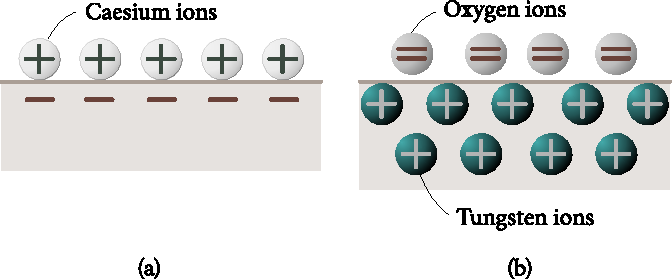
\includegraphics[scale=0.95]{figures/cap_08/fig_8_3.pdf}
		\caption[]{}
		\label{fig:8_3}
	\end{center}
	\vspace{-0.8cm}
\end{figure}

\textbf{The Length of Bodies in Different Frames.} Let us consider a rod arranged along the $x'$-axis and at rest relative to the reference frame K$'$ (\fig{8_3}). Its length in this frame is $l_0=x_2'-x_1'$ where $x_1'$ and $x_2'$ are the coordinates of the rod ends that do not change with the time $t'$. The rod travels with the velocity $v=v_0$ relative to the frame K. To determine its length in this frame, we must note the coordinates of the rod ends $x_1$ and $x_2$ at the same moment $t_1=t_2=b$. Their difference $l=x_2-x_1$ will give the length of the rod measured in the frame K. To find the relationship between $l_0$ and $l$, we must take the equation of the Lorentz transformations that contains $x'$, $x$, and $t$, \ie, the first of the equations~\eqref{eq:8_17}. Substituting $v0/c$ for $\beta$ in this equation, we obtain 
\begin{equation*}
	x_1' = \frac{x_1 - v_0 b}{\left[1 - \left(v_0^2/c^2\right)\right]^{1/2}},\quad x_2' = \frac{x_2 - v_0 b}{\left[1 - \left(v_0^2/c^2\right)\right]^{1/2}}
\end{equation*}

\noindent
whence
\begin{equation*}
	x_2' - x_1' = \frac{x_2 - x_1}{\left[1 - \left(v_0^2/c^2\right)\right]^{1/2}}.
\end{equation*}

\noindent
Using the symbols $l$ and $l_0$ and also replacing the relative velocity of the reference frames $v_0$ with the velocity $v$ of the rod the frame K that equals it, we arrive at the expression
\begin{equation}\label{eq:8_19}
	l = l_0 \left(1 - \frac{v_0^2}{c^2}\right)^{1/2}.
\end{equation}

\noindent
Thus, the length of the rod $l$ measured in a frame relative to which it is moving is shorter than the length $l_0$ measured in the frame relative to which the rod is at rest.\footnote{The length $l_0$ measured in the frame relative to which the rod is at rest is called the \textbf{proper length} of the rod.}

If a rod of length $l_0=x2-x1$ is at rest relative to the frame K, then to determine its length in the frame K$'$ we must note the coordinates of its ends $x_1'$ and $x_2'$ at the same moment $t_1'=t_2'=b$. The difference $l=x_2'-x_1'$ gives the length of the rod in the frame K$'$ relative to which it is moving with the velocity $v$. Using the first of the equations~\eqref{eq:8_16}, we again arrive at \eqn{8_19}.

It must be noted that the dimensions of the rod are identical in all the reference frames in the direction of the axes $y$ and $z$.

Thus, in moving bodies, their dimensions contract in the direction of their motion the greater, the higher is the velocity. This phenomenon is called the \textbf{Lorentz} (or \textbf{Fitzgerald}) contraction. It is interesting to note that the change in the shape of bodies even at velocities comparable with $c$ cannot be detected visually (or in a photograph). The reason is very simple. When observing visually or photographing a body, we register light pulses from different points of the body that reach the retina of our eye or the photographic plate simultaneously. These pulses, however, are not emitted simultaneously. The pulses from the more remote sections were emitted before those from the nearer sections. Thus, if the body is moving, a distorted image of it is formed on the retina of the eye or on the photograph. The relevant calculations show that this distortion will result in compensation of the Lorentz contraction\footnote{If there were no Lorentz contraction, rapidly moving bodies ought to seem extended in the direction of their motion.} so that the bodies seem to be only turned instead of distorted. Consequently, a spherically shaped body even at high velocities will be perceived visually as a body with a spherical configuration.

\textbf{Length of Time Between Events.} Let us suppose that two events occur at the same point of the frame K$'$. The coordinate $x_1'=a$ and the moment $t_1'$ correspond to the first event in this frame, and the coordinate $x_2'=a$ and the moment $t_2'$ to the second one. According to the last of the equations~\eqref{eq:8_16}, the moments corresponding to these events in the frame K will be (we have introduced $v_0/c$ instead of $\beta$)
\begin{equation*}
	t_1 = \frac{t_1' + (v_0/c)^2 a}{\left[1 - \left(v_0^2/c^2\right)\right]^{1/2}},\quad t_2 = \frac{t_2' + (v_0/c^2) a}{\left[1 - \left(v_0^2/c^2\right)\right]^{1/2}}.
\end{equation*}

\noindent
Hence,
\begin{equation*}
	t_2 - t_1 = \frac{t_2' - t_2'}{\left[1 - \left(v_0^2/c^2\right)\right]^{1/2}}.
\end{equation*}

Introducing the notation $t_2-t_1=\Delta t$ and $t_2'-t_1'=\Delta t'$ , we get the equation
\begin{equation}\label{eq:8_20}
	\Delta t = \frac{\Delta t'}{\left[1 - \left(v_0^2/c^2\right)\right]^{1/2}}
\end{equation}

\noindent
that relates the lengths of time between two events measured in the frames K and K$'$. We remind our reader that in the frame K$'$ both events occur at the same point, \ie, $x_1'=x_2'$.

Assume that both events occur with the same particle that is at rest in the frame K$'$ and is moving relative to the frame K with the velocity $v=v_0$. Therefore, $\Delta t'$ can be interpreted as the length of time measured on a clock that is stationary relative to the particle, or, in other words, measured on a clock that is moving together with the particle (we have in mind motion relative to the frame K). The time measured on a clock moving together with a body is called the \textbf{proper time} of this body and is usually denoted by the symbol $\tau$. Thus, $\Delta t' = \Delta\tau$. We can thus write \eqn{8_20} as follows:
\begin{equation}\label{eq:8_21}
	\Delta\tau = \Delta t \left[1 - \left(v^2/c^2\right) \right]^{1/2}
\end{equation}

\noindent
(we have replaced the relative velocity of the reference frames $v_0$ with the velocity of the particle $v$ equal to it).

Equation~\eqref{eq:8_21} relates the proper time of a body $\tau$ to the time $t$ read on a clock of a reference frame relative to which the body is moving with the velocity $v$ (this clock itself is moving relative to the body with the velocity $-v$).

A glance at \eqn{8_21} shows that the proper time is always smaller than the time measured on a clock moving relative to a body (in the latter case the effect called \textbf{time dilation} is observed). We shall show in the following section that the proper time is an invariant (\ie, is identical in all reference frames).

Considering the events occurring with the particle in the frame K, we can define $\Delta t$ as the length of time measured on a stationary clock, and $\Delta\tau$ as the length of time measured on a clock moving with the velocity $v$. By \eqn{8_21}, we have $\Delta\tau<\Delta t$. We can therefore say that the moving clock runs slower than the clock at rest (it must not be forgotten that in all respects except for their velocity the clocks are absolutely identical).

Equation~\eqref{eq:8_21} has been directly confirmed experimentally. Cosmic rays contain particles called mu-mesons or muons. These particles are unstable and decay spontaneously into an electron (or positron) and two neutrinos. The mean lifetime of muons measured in conditions when they are stationary (or are moving with a low velocity) is about \SI{2e-6}{\second}. It would seem that even when travelling with the speed of light, muons could cover a distance of only about \SI{600}{\metre}. As observations show, however, muons are formed in cosmic rays at an altitude of from \SIrange{20}{30}{\kilo\metre}, and a considerable number of them manage to reach the Earth's surface. The explanation is that \SI{2e-6}{\second} is the proper lifetime of a muon, \ie, time measured on a clock travelling together with it. The time according to the clock of an observer on the Earth will be much greater [see \eqn{8_21}; $v$ of a muon is close to $c$]. It is therefore not surprising that the observer registers a distance travelled by a muon much greater than \SI{600}{\metre}. We must note that from the position of an observer travelling together with a muon, the distance it covers to the Earth's surface contracts to \SI{600}{\metre} [see \eqn{8_19}], so that the muon manages to travel this distance in \SI{2e-6}{\second}.

\section{Interval}\label{sec:8_4}

We pointed out in Sec.~\ref{sec:8_1} that a world point with the coordinates $ct, x, y, z$ can be associated with every event in imaginary four-dimensional space. Let one event have the coordinates $ct_1, x_1, y_1, z_1$ and another the coordinates $ct_2, x_2, y_2, z_2$. We shall introduce the notation $t_2-t_1=\Delta t$, $x_2-x_1=\Delta x$, etc.

We remind our reader that owing to the qualitative distinction between time and space, the square of the difference between the time coordinates $(c\Delta t)^2$ and the squares of the differences between the space coordinates $\Delta x^2, \Delta y^2, \Delta z^2$ enter the expression for the square of the ``distance'' between events (more exactly, between the world points corresponding to the events) with opposite signs:
\begin{equation}\label{eq:8_22}
	\Delta s^2 = c^2\Delta t^2 - \Delta x^2 - \Delta y^2 - \Delta z^2.
\end{equation}

\noindent
The quantity $\Delta s$ determined by this equation is defined as the \textbf{interval} between events.

Introducing the distance $\Delta l=\left(\Delta x^2+\Delta y^2+\Delta z^2\right)^{1/2}$ between the points of conventional three-dimensional space at which the events being considered occurred, the expression for the interval can be written in the form
\begin{equation}\label{eq:8_23}
	\Delta s = \left(c^2\Delta t^2 - \Delta l^2\right)^{1/2}.
\end{equation}

It is easy to convince ourselves that the interval between two given events is the same in all inertial reference frames. It is exactly this circumstance that served as the grounds to consider it the analogue of the distance $\Delta l$ between two points in conventional three-dimensional space ($\Delta l$ does not change its value when we pass over from one three-dimensional reference frame to another).

Assume that in the reference frame K the square of the interval is determined by \eqn{8_22}. The square of the interval between the same events in the frame K$'$ is
\begin{equation}\label{eq:8_24}
	\Delta s'^2 = c^2\Delta t'^2 - \Delta x'^2 - \Delta y'^2 - \Delta z'^2.
\end{equation}

\noindent
By Eqs.~\eqref{eq:8_17}
\begin{equation*}
	\Delta x' = \frac{\Delta x - \beta c\Delta t}{\left(1 - \beta^2\right)^{1/2}},\quad \Delta y' = \Delta y,\quad \Delta z' = \Delta z,\quad 	\Delta t' = \frac{\Delta t - (\beta/c)\Delta x}{\left(1 - \beta^2\right)^{1/2}}.
\end{equation*}

\noindent
Introducing these values into \eqn{8_24}, after simple transformations we find that $\Delta s'^2 = c^2\Delta t^2 - \Delta x^2 - \Delta y^2 - \Delta z^2$, \ie, that
\begin{equation*}
	\Delta s'^2 = \Delta s^2.
\end{equation*}

The interval is thus invariant with respect to a transition from one inertial reference frame to another. We saw in the preceding section that the lengths of time $\Delta t$ and lengths $\Delta l$ are not invariant with respect to such a transition. Hence, each of the addends forming the quantity $\Delta s^2=c^2\Delta t^2-\Delta l^2$ changes in a transition from one frame to another; the quantity $\Delta s^2$ itself remains unchanged.

The interval between two events occurring with a particle is in a simple relation with the length of the proper time between these events. By \eqn{8_21}, the length of the proper time $\Delta\tau$ is related to the time $\Delta t$ measured on a clock of the frame relative to which the particle is travelling with the velocity $v$ by the expression
\begin{equation*}
	\Delta\tau = \Delta t\left(1 - \frac{v^2}{c^2}\right).
\end{equation*}

\noindent
Let us transform this equation as follows:
\begin{equation*}
	\Delta\tau = \frac{1}{c}\left[c^2\Delta t^2 - (v\Delta t)^2\right]^{1/2} = \frac{1}{c}\left(c^2\Delta t^2 - \Delta l^2\right)^{1/2}.
\end{equation*}

\noindent
Here $\Delta l=v\Delta t$ is the distance travelled by the particle during the time $\Delta t$. A comparison with \eqn{8_23} shows that
\begin{equation}\label{eq:8_25}
	\Delta\tau = \frac{1}{c}\Delta s
\end{equation}

\noindent
where $\Delta s$ is the interval between events separated by the time $\Delta\tau$.

It follows from \eqn{8_25} that the length of the proper time is proportional to the interval between events. The interval is an invariant. Consequently, the proper time is also an invariant, \ie, does not depend on the reference frame in which the motion of a given body is being observed.

According to \eqn{8_23}, the interval may be real (if $c\Delta t>\Delta l$) or imaginary (if $c\Delta t<\Delta l$). In a particular case, the interval may equal zero (if $c\Delta t=\Delta l$). The last case occurs for events consisting in the emission of a light signal from the point $x_1, y_1, z_1$ at the moment $t_1$ and in the arrival of this signal at the point $x_2, y_2, z_2$ at the moment $t_2$. Since here $\Delta l=c\Delta t$, the interval between the events equals zero.

Owing to its invariance, an interval that is real (or imaginary) in a reference frame K will be real (or imaginary) in any other inertial frame K$'$.

For a real interval, we have
\begin{equation*}
	c^2\Delta t^2 - \Delta l^2 = c^2\Delta t^2 - \Delta l'^2 > 0.
\end{equation*}

\noindent
It can be seen from this expression that we can find a frame K$'$ in which $\Delta l'=0$, \ie, both events will coincide in space. No reference frame exists, however, in which $\Delta t'=0$ (the interval would become imaginary at such a value of $\Delta t'$). Thus, events separated by a real interval cannot become simultaneous in any reference frame. For this reason, real intervals are called \textbf{timelike}.

We must note that events occurring with the same particle (we have in mind a particle with a rest mass differing from zero) can be separated only by a timelike interval. Indeed, the velocity of such a particle $v$ is always lower than $c$. Hence, the path $\Delta l$ travelled by the particle is less than $c\Delta t$, whence it follows that $\Delta s^2>0$. According to the last of the equations~\eqref{eq:8_17}, we have
\begin{equation}\label{eq:8_26}
	\Delta t' = \frac{\Delta t - (\beta/c) \Delta x}{\left(1 - \beta^2\right)^{1/2}}.
\end{equation}

\noindent
If $\Delta x$ and $\Delta x$ separate events occurring with the same particle, then $\Delta x/\Delta t$ gives the component $v_x$ of the particle's velocity. Therefore, \eqn{8_26} in this condition can be written in the form
\begin{equation*}
	\Delta t' = \frac{\Delta t - (\beta/c)(\Delta x/\Delta t)\Delta t}{\left(1 - \beta^2\right)^{1/2}} = \frac{\Delta t}{\left(1 - \beta^2\right)^{1/2}}\left(1 - \beta \frac{v_x}{c}\right).
\end{equation*}

\noindent
Since both $\beta=v_0/c$ and $v_x/c$ are less than unity, the quantity in parentheses in the right-hand side of the equation is positive for all frames K$'$. Hence, it follows that $\Delta t'$ and $\Delta t$ have the same signs. This signifies that two events occurring with a particle take place in the same sequence in all frames. For example, the birth of a particle in all reference frames precedes its decay.

For an imaginary interval, we have
\begin{equation*}
	c^2\Delta t^2 - \Delta l^2 = c^2\Delta t'^2 - \Delta '^2 > 0.
\end{equation*}

\noindent
This shows that we can find a frame K$'$ in which $\Delta t'=0$, \ie, both events occur at the same moment $t'$. No reference frame exists, however, in which we would have $\Delta l'=0$ (the interval would be real with such a value of $\Delta l'$). Thus, events separated by an imaginary interval cannot coincide in space in any reference frame. For this reason, imaginary intervals are called \textbf{spacelike}.

The distance $\Delta l$ between points at which events separated by a spacelike interval occur exceeds $c\Delta t$. Therefore, these events cannot in any way affect each other, \ie, cannot be causally related to each other (we remind our reader that no actions exist which propagate at a velocity exceeding $c$).

Causally related events can be separated only by a timelike or a zero interval.

\section{Transformation and Addition of Velocities}\label{sec:8_5}

Let us consider the motion of a point particle. The position of the particle in the frame K is determined at each moment $t$ by the coordinates $x, y, z$. The expressions
\begin{equation*}
	v_x = \diffin{x}{t},\quad v_y = \diffin{y}{t},\quad v_z = \diffin{z}{t}
\end{equation*}

\noindent
are the projections of the vector of the particle's velocity relative to the frame K onto the axes $x, y, z$. The position of the particle in the frame K$'$ is characterized at each moment $t'$ by the coordinates $x', y', z'$. The projections of the vector of the particle's velocity relative to the frame K$'$ onto the axes $x', y', z'$ are determined by the expressions
\begin{equation*}
	v_x' = \diffin{x'}{t'},\quad v_y' = \diffin{y'}{t'},\quad v_z' = \diffin{z'}{t'}.
\end{equation*}

From Eqs.~\eqref{eq:8_16}, we have
\begin{equation*}
	\deriv{x} = \frac{\deriv{x'}+v_0\deriv{t'}}{\left(1-v_0^2/c^2\right)^{1/2}},\quad \deriv{y} = \deriv{y'},\quad \deriv{z} = \deriv{z'},\quad \deriv{t} = \frac{\deriv{t'}+(v_0/c^2)\deriv{x'}}{\left(1-v_0^2/c^2\right)^{1/2}}
\end{equation*}

\noindent
(we have replaced $\beta$ with $v_0/c$). Dividing the first three equations by the fourth one, we get formulas for transformation of the velocities when passing over from one reference frame to another:
\begin{equation}\label{eq:8_27}
	v_x = \frac{v_x'+v_0}{1 - v_0v_x'/c^2},\quad  v_y = \frac{v_y'\left(1-v_0^2/c^2\right)^{1/2}}{1 - v_0v_x'/c^2},\quad v_z = \frac{v_z'\left(1-v_0^2/c^2\right)^{1/2}}{1 - v_0v_x'/c^2}.
\end{equation}

\noindent
When $v_0\ll c$, equations~\eqref{eq:8_27} become the same as the velocity addition equations~\eqref{eq:2_20} of classical mechanics.

It is simple to obtain expressions for velocities in the frame K$'$ through the velocities in the frame K from Eqs.~\eqref{eq:8_17}:
\begin{equation}\label{eq:8_28}
	v_x' = \frac{v_x-v_0}{1 - v_0v_x/c^2},\quad  v_y' = \frac{v_y\left(1-v_0^2/c^2\right)^{1/2}}{1 - v_0v_x/c^2},\quad v_z' = \frac{v_z\left(1-v_0^2/c^2\right)^{1/2}}{1 - v_0v_x/c^2}.
\end{equation}

\noindent
These equations differ from equations~\eqref{eq:8_27} only in the sign before $v_0$. This result could naturally be predicted.

If a body is travelling parallel to the $x$-axis, its velocity $v$ relative to the frame K coincides with $v_x$, and its velocity $v'$ relative to the frame K$'$ coincides with $v_x'$. In this case, the law of velocity addition has the form
\begin{equation}\label{eq:8_29}
	v = \frac{v' + v_0}{1 + v_0 v'/c^2}.
\end{equation}

\noindent
Assume that the velocity $v'$ equals $c$. Hence, \eqn{8_29} gives us the following value for $v$:
\begin{equation*}
	v = \frac{c + v_0}{1 + v_0 c/c^2} = c.
\end{equation*}

\noindent
This result is not surprising because the Lorentz transformations (and, consequently, the velocity addition equations too) are based on the assertion that the speed of light is the same in all reference frames. Assuming in \eqn{8_29} that $v'=v_0=c$, we also get a value of $c$ for $v$. Thus, if the velocities $v'$ and $v_0$ being added do not exceed $c$, then the resultant velocity $v$ also cannot exceed $c$.

\section{Relativistic Expression for the Momentum}\label{sec:8_6}

Newton's equations are invariant with respect to the Galilean transformations (see Sec.~\ref{sec:2_7}). They are not invariant, however, with respect to the Lorentz transformations. In particular, the law of momentum conservation (see Sec.~\ref{sec:3_10}) following from Newton's laws is not invariant with respect to the Lorentz transformations. To convince ourselves in the truth of this statement, let us see what a completely inelastic collision of two identical balls of mass $m$ is like in the frames K and K$'$ (\fig{8_4}).

\begin{figure}[t]
	\begin{center}
		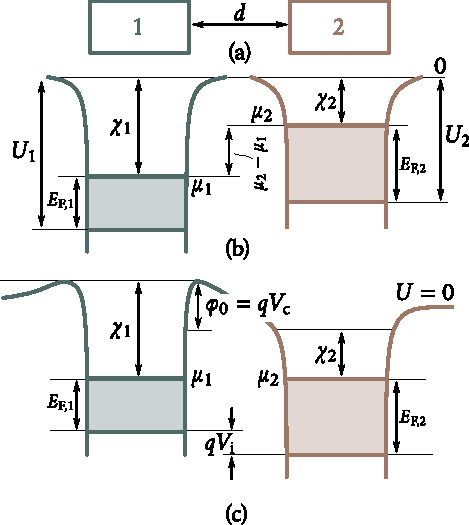
\includegraphics[scale=0.95]{figures/cap_08/fig_8_4.pdf}
		\caption[]{}
		\label{fig:8_4}
	\end{center}
	\vspace{-0.8cm}
\end{figure}

Assume that the balls are moving toward each other in the frame K along the $x$-axis with velocities identical in magnitude whose projections onto the $x$-axis are $v_{x1}=v_0$ and $v_{x2}=-v_0$ ($v_0$ is the relative velocity of the frames K and K$'$). In these conditions, the balls will be at rest after colliding: $v_{x1}=v_{x2}=0$. Thus, the total momentum of the system both before and after the collision equals zero---the momentum in the frame K is conserved.

Let us now consider the same process in the frame K$'$. Using the first of the equations~\eqref{eq:8_28}, we find for the velocities of the balls before they collide the values $v{x1}'=0$ and $v{x2}'=-2v_0/(1+v_0^2/c^2)$, and for the velocities of the balls after they collide the same value $c_{x1}'=v{x2}'=-v_0$. Therefore, the total momentum before the collision is $-2mv_0/(1+v_0^2/c^2)$, and after the collision is $-2mv_0$. If $v_0\ll c$, the momentum of the system before and after the collision is virtually the same. When the balls are travelling with a great velocity $v_0$, however, the difference between the initial and the final momenta becomes quite appreciable. Thus, using the Newtonian expression for the momentum, we arrived at the conclusion that the momentum does not seem to be conserved in the frame K$'$. One of the fundamental laws of mechanics---the law of momentum conservation---is not invariant with respect to the Lorentz transformations in the Newtonian formulation.

It can be shown that the law of momentum conservation will be invariant with respect to the Lorentz transformations at any velocities if we substitute the proper time of a particle $\tau$ for the time $t$ in the classical expression
\begin{equation}\label{eq:8_30}
	\vec{p} = m\vec{v} = m\diff{\vec{r}}{t}.
\end{equation}

\noindent
Consequently, the relativistic expression for the momentum has the form
\begin{equation}\label{eq:8_31}
	\vec{p} = m\diff{\vec{r}}{\tau}.
\end{equation}

\noindent
When $v\ll c$, the length of the proper time of a particle $\deriv{\tau}$ does not virtually differ from the length $\deriv{t}$ measured according to the clock of the frame in which the motion of the particle is being considered [see \eqn{8_21}]. Hence, \eqn{8_31} transforms into the classical expression~\eqref{eq:8_30}.

Remember that $\deriv{\vec{r}}$ in \eqn{8_31} is the displacement of the particle in the reference frame in which the momentum $\vec{p}$ is determined, whereas the length of time $\deriv{\tau}$ is determined on a clock travelling together with the particle.

We get an expression for the momentum through the time $t$ of the frame of reference relative to which the motion of bodies is being observed. By \eqn{8_21}, we have $\deriv{\tau}=\deriv{t}\left(1-v^2/c^2\right)^{1/2}$, where $v$ is the velocity of the body. This substitution in \eqn{8_31} yields
\begin{equation*}
	\vec{p} = \frac{m}{\left(1-v^2/c^2\right)^{1/2}}\diff{\vec{r}}{t}
\end{equation*}

\noindent
or, since $\diffin{\vec{r}}{t}=\vec{v}$:
\begin{equation}\label{eq:8_32}
	\vec{p} = \frac{m\vec{v}}{\left(1-v^2/c^2\right)^{1/2}}.
\end{equation}

The mass $m$ in \eqn{8_32} is invariant and, consequently, does not depend on the velocity of the body.

It can be seen from \eqn{8_32} that the velocity dependence of the momentum is more complicated than is assumed in Newtonian mechanics. When $v\ll c$, \eqn{8_32} transforms into the Newtonian expression $\vec{p}=m\vec{v}$.

We must note that \eqn{8_32} permits the following interpretation to be made, which is gradually losing favour. The momentum, as in Newtonian mechanics, equals the product of the mass of a body and its velocity:
\begin{equation}\label{eq:8_33}
	\vec{p} = m_{\text{r}}\vec{v}.
\end{equation}

\noindent
The mass of a body, however, is not a constant invariant quantity, but depends on the velocity according to the law
\begin{equation}\label{eq:8_34}
	m_{\text{r}} = \frac{m}{\left(1-v^2/c^2\right)^{1/2}}.
\end{equation}

\noindent
In this interpretation, the invariant mass $m$ is called the \textbf{rest mass} (it is often denoted by the symbol $m_0$). The non-invariant mass $m_{\text{r}}$ depending on the velocity is called the \textbf{relativistic mass}.

\section{Relativistic Expression for the Energy}\label{sec:8_7}

Newton's second law states that the time derivative of the momentum of a particle (point particle) equals the resultant force acting on the particle [see \eqn{2_10}]. The equation of the second law is invariant relative to the Lorentz transformations if by the momentum we understand the quantity~\eqref{eq:8_32}. Hence, the relativistic expression of Newton's second law has the form
\begin{equation}\label{eq:8_35}
	\frac{\upd}{\deriv{t}}\left[\frac{m\vec{v}}{\left(1-v^2/c^2\right)^{1/2}}\right] = \vec{F}.
\end{equation}

It should be borne in mind that the equation $m\vec{a}=\vec{F}$ cannot be used in the relativistic case, the acceleration $\vec{a}$ and the force $\vec{F}$, generally speaking, being non-collinear.

We shall note that neither the momentum nor the force are invariant quantities. Equations for the transformation of the momentum components when passing over from one inertial reference frame to another will be obtained in the following section. We give the equations for transformation of the force components without deriving them:
\begin{equation}\label{eq:8_36}
	F_x = \frac{F_x' + (\beta/c)\vec{F}'\vec{\cdot}\vec{v}'}{1 + \beta(v_x'/c)},\quad F_y = \frac{F_y'\left(1-\beta^2\right)^{1/2}}{1 + \beta(v_x'/c)},\quad F_z = \frac{F_z'\left(1-\beta^2\right)^{1/2}}{1 + \beta(v_x'/c)}
\end{equation}

\noindent
(here $\beta=v_0/c$ and $\vec{v}'$ is the velocity of a particle in the frame K'). If in the frame K$'$ the force $\vec{F}'$ acting on a particle is perpendicular to the velocity of the particle $\vec{v}'$, the scalar product $\vec{F}'\vec{\cdot}\vec{v}'$ equals zero, and the first of the equations~\eqref{eq:8_36} is simplified as follows
\begin{equation}\label{eq:8_37}
	F_x = \frac{F_x'}{1 + \beta(v_x'/c)}.
\end{equation}

\noindent
To find the relativistic expression for the energy, let us proceed in the same way as we did in Sec.~\ref{sec:3_2}. We shall multiply \eqn{8_35} by the displacement of a particle $\deriv{s}=\vec{v}\,\deriv{t}$. The result is
\begin{equation*}
	\frac{\upd}{\deriv{t}}\left[\frac{m\vec{v}}{\left(1-v^2/c^2\right)^{1/2}}\right]\vec{v}\,\deriv{t} = \vec{F}\,\deriv{\vec{s}}.
\end{equation*}

\noindent
The right-hand side of this equation gives the work $\deriv{A}$ done on the particle during the time $\deriv{t}$. We saw in Sec.~\ref{sec:3_2} that the work of the resultant of all the forces is spent on an increment of the kinetic energy of the particle [see \eqn{3_11}]. Consequently, the left-hand side of the equation should be interpreted as the increment of the kinetic energy $E_{\text{k}}$ of the particle during the time $\deriv{t}$. Thus,
\begin{equation*}
	\deriv{E_{\text{k}}} = \frac{\upd}{\deriv{t}}\left[\frac{m\vec{v}}{\left(1-v^2/c^2\right)^{1/2}}\right]\vec{\cdot}\vec{v}\,\deriv{t} = \vec{v}\vec{\cdot} \upd\left[\frac{m\vec{v}}{\left(1-v^2/c^2\right)^{1/2}}\right].
\end{equation*}

Let us transform the obtained expression, bearing in mind that $\vec{v}\vec{\cdot}\deriv{\vec{v}}=\deriv{(\vec{v}^2/2)}$ [see \eqn{1_54}]:
\begin{align*}
	\deriv{E_{\text{k}}} &= \vec{v}\vec{\cdot} \left[\frac{m\,\deriv{\vec{v}}}{\left(1-v^2/c^2\right)^{1/2}} +  \frac{m\vec{v}(\vec{v}\vec{\cdot}\,\deriv{\vec{v}}/c^2)}{\left(1-v^2/c^2\right)^{3/2}}\right]\\
	& = \frac{m\,\deriv{(v^2/2)}}{\left(1-v^2/c^2\right)^{3/2}} = \frac{mc^2\deriv{v^2/c^2}}{2\left(1-v^2/c^2\right)^{3/2}} = \upd\left[\frac{mc^2}{\left(1-v^2/c^2\right)^{1/2}}\right].
\end{align*}

\noindent
Integration of this expression yields
\begin{equation}\label{eq:8_38}
	E_{\text{k}} = \frac{mc^2}{\left(1-v^2/c^2\right)^{1/2}} + \text{constant}.
\end{equation}

\noindent
According to the meaning of kinetic energy, it must vanish when $v=0$. We thus get a value of $-mc^2$ for the constant. Hence, the relativistic expression for the kinetic energy of a particle has the form
\begin{equation}\label{eq:8_39}
	E_{\text{k}} = \frac{mc^2}{\left(1-v^2/c^2\right)^{1/2}} - mc^2 = mc^2\left[\frac{1}{\left(1-v^2/c^2\right)^{1/2}} - 1\right].
\end{equation}

For small velocities ($v\ll c$), \eqn{8_39} can be transformed as follows:
\begin{equation*}
	E_{\text{k}} = mc^2 \left[\frac{1}{\left(1-v^2/c^2\right)^{1/2}} - 1\right]\approx mc^2\left(1 + \frac{1}{2}\frac{v^2}{c^2} - 1\right) = \frac{1}{2}mv^2.
\end{equation*}

\noindent
We have arrived at the Newtonian expression for the kinetic energy of a particle. This is what should be expected because for velocities much smaller than the speed of light all the equations of relativistic mechanics must transform into the relevant equations of Newtonian mechanics.

Let us consider a free particle (\ie, one that does not experience the action of external forces) travelling with the velocity $v$. We have learned that this particle has a kinetic energy determined by \eqn{8_39}. We have grounds, however (see below), to ascribe the additional energy equal to
\begin{equation}\label{eq:8_40}
	E_0 = mc^2
\end{equation}

\noindent
to a free particle in addition to the kinetic energy~\eqref{eq:8_39}. Thus, the total energy of a free particle is determined by the expression $E=E_{\text{k}}+E_0=E_{\text{k}}+mc^2$. With a view to \eqn{8_39}, we find that
\begin{equation}\label{eq:8_41}
	E = \frac{mc^2}{\left(1-v^2/c^2\right)^{1/2}}.
\end{equation}

When $v=0$, \eqn{8_41} transforms into \eqn{8_40}. This is why $E_0=mc^2$ is called the rest energy. This energy is the internal energy of a particle not associated with its motion as a whole. Equations~\eqref{eq:8_40} and~\eqref{eq:8_41} hold not only for an elementary particle, but also for a complicated body consisting of many particles. The energy $E_0$ of such a body includes, apart from the rest energies of its particles, the kinetic energy of these particles (due to their motion relative to the body's centre of mass) and the energy of their interaction with one another. The rest energy, like the total\footnote{We shall note here that the term ``total energy'' has a different meaning in relativistic mechanics than in Newtonian mechanics. In the latter, the total energy is defined as the sum of the kinetic and potential energies of a particle. In relativistic mechanics, by the total energy is meant the sum of the kinetic and rest energies of a particle.} energy~\eqref{eq:8_41}, does not include the potential energy of a body in an external force field.

Eliminating the velocity $v$ from Eqs.~\eqref{eq:8_32} and~\eqref{eq:8_41} [\eqn{8_32} should be taken in the scalar form], we obtain an expression giving the total energy of a particle through its momentum p:
\begin{equation}\label{eq:8_42}
	E = c\left(p^2 + m^2c^2\right)^{1/2}.
\end{equation}

\noindent
When $p\ll mc$, this equation can be written in the form
\begin{equation}\label{eq:8_43}
	E = mc^2\left[1 + \left(\frac{p}{mc}\right)^2\right]\approx mc^2\left[1 + \left(\frac{1}{2}\frac{p}{mc}\right)^2\right] = mc^2 + \frac{p^2}{2m}.
\end{equation}

\noindent
The expression obtained differs from Newton's equation for the kinetic energy $E_{\text{k}}=p^2/(2m)$ in the addend $mc^2$.

It must be noted that the following equation results from a comparison of Eqs.~\eqref{eq:8_32} and~\eqref{eq:8_41}:
\begin{equation}\label{eq:8_44}
	\vec{p} = \frac{E}{c^2}\vec{v}.
\end{equation}

We shall explain why the energy~\eqref{eq:8_41}, and not only the kinetic energy~\eqref{eq:8_39}, should be ascribed to a free particle. Energy according to its meaning must be a conserved quantity. The relevant treatment shows that when particles collide, the sum (for the particles) of expressions of the form of \eqn{8_41} is conserved, whereas the sum of Eqs.~\eqref{eq:8_39} is not conserved. It is impossible to comply with the requirement of energy conservation in all inertial reference frames if we do not include the rest energy~\eqref{eq:8_40} in the total energy.

In addition, we succeed in forming an invariant, \ie, a quantity that does not change in the Lorentz transformations, from \eqn{8_41} for the energy and~\eqref{eq:8_42} for the momentum. Indeed, it can be seen from \eqn{8_42} that
\begin{equation}\label{eq:8_45}
	\frac{E^2}{c^2} - p^2 = m^2c^2 = \text{inv}
\end{equation}

\noindent
(we remind our reader that the mass $m$ and speed $c$ are invariant quantities). Experiments with fast particles confirm the invariance of the quantity in \eqn{8_45}. If by $E$ in \eqn{8_45} we understand the kinetic energy~\eqref{eq:8_39}, then \eqn{8_45} will not be invariant.

Let us obtain another expression for the relativistic energy. From \eqn{8_21}, we find that
\begin{equation}\label{eq:8_46}
	\frac{1}{\left(1 - v^2/c^2\right)^{1/2}} = \diff{t}{\tau}
\end{equation}

\noindent
where $\deriv{t}$ is the time that elapses between two events occurring with a particle and measured on a clock of the reference frame relative to which the particle is travelling with the velocity $v$, while $\deriv{\tau}$ is the same time measured on a clock travelling together with the particle (proper time). Using \eqn{8_46} in \eqn{8_41} we get the expression 
\begin{equation}\label{eq:8_47}
	E = mc^2\,\diff{t}{\tau}.
\end{equation}

\noindent
We shall use this equation in the following section.

\section{Transformations of Momentum and Energy}\label{sec:8_8}

The total energy $E$ and momentum $p$ are not invariants. Indeed, both quantities depend on $v$, while the latter has different values in different reference frames. Let us see how the energy and momentum transform when we pass over from one reference frame to another.

Consider an elementary displacement of a particle. Assume that in the reference frame K this displacement occurs during the time $\deriv{t}$, and its components are $\deriv{x}, \deriv{y}, \deriv{z}$. In the frame K$'$, the same displacement occurs during the time $\deriv{t'}$, and its components are $\deriv{x'}, \deriv{y'}, \deriv{z'}$. According to Eqs.~\eqref{eq:8_18}, the following relations hold between the lengths of time and the components of the displacement:
\begin{equation*}
	\deriv{x} = \frac{\deriv{x'}+\beta c\,\deriv{t'}}{\left(1 - \beta^2\right)^{1/2}},\quad \deriv{y}=\deriv{y'},\quad \deriv{z}=\deriv{z'},\quad c\,\deriv{t} = \frac{c\,\deriv{t'}+\beta\,\deriv{x'}}{\left(1 - \beta^2\right)^{1/2}}.
\end{equation*}

Let us multiply these equations by the mass of the particle $m$ and divide them by the proper time of the particle $\deriv{\tau}$ corresponding to the lengths of time $\deriv{t}$ and $\deriv{t'}$ (it should be remembered that the mass and the proper time are invariant quantities, \ie, have the same value in both frames). As a result, we get
\begin{equation}\label{eq:8_48}
	\begin{split}
	&m\,\diff{x}{\tau} = \frac{m(\diffin{x'}{\tau})+\beta mc(\diffin{t'}{\tau})}{\left(1 - \beta^2\right)^{1/2}},\quad m\,\diff{y}{\tau} = m\,\diff{y'}{\tau},\\
	&m\,\diff{z}{\tau} = m\,\diff{z'}{\tau},\quad mc\,\diff{t}{\tau} = \frac{mc(\diffin{t'}{\tau})+\beta m(\diffin{x'}{\tau})}{\left(1 - \beta^2\right)^{1/2}}.
	\end{split}
\end{equation}

By \eqn{8_31}, we have $m\,(\diffin{x}{\tau})=p_x, m\,(\diffin{x'}{\tau})=p_x', m\,(\diffin{y}{\tau})=p_y$, etc. According to \eqn{8_47}, we have $mc\,(\diffin{t}{\tau})=E/c$, and $mc\,(\diffin{t'}{\tau})=E'/c$. Hence, Eqs.~\eqref{eq:8_48} can be written in the form
\begin{equation}\label{eq:8_49}
	p_x = \frac{p_x'+\beta(E'/c)}{\left(1 - \beta^2\right)^{1/2}},\quad p_y = p_y',\quad p_z = p_z',\quad \frac{E}{c} = \frac{(E'/c)+\beta p_x'}{\left(1 - \beta^2\right)^{1/2}}.
\end{equation}

We have obtained equations by means of which the momentum and energy of a particle are transformed when we pass over from one inertial reference frame to another. These equations coincide with Eqs.~\eqref{eq:8_18} used to transform the coordinates and time. To facilitate a comparison, let us write Eqs.~\eqref{eq:8_18} and~\eqref{eq:8_49} side by side:
\begin{equation}\label{eq:8_50}
	\begin{split}
		&x = \frac{x'+\beta(ct')}{\left(1 - \beta^2\right)^{1/2}},\quad y=y',\quad z=z',\quad (ct) = \frac{(ct')+\beta x'}{\left(1 - \beta^2\right)^{1/2}}\\
		&p_x = \frac{p_x'+\beta(E'/c)}{\left(1 - \beta^2\right)^{1/2}},\quad p_y = p_y',\quad p_z = p_z',\quad \frac{E}{c} = \frac{(E'/c)+\beta p_x'}{\left(1 - \beta^2\right)^{1/2}}.
	\end{split}
\end{equation}

\noindent
It follows from the comparison that the components of the momentum behave in transformations like coordinates, and the energy like time.

The analogy disclosed by Eqs.~\eqref{8_50} allows us to present the mathematics of relativistic mechanics in the form of relations between vectors in an imaginary four-dimensional space (four-vectors). We have already noted in Sec.~\ref{sec:8_1} that we have to ascribe unusual properties to this space which differ from the properties of the Euclidean space we are accustomed to. In three-dimensional Euclidean space, the quantity
\begin{equation*}
	\Delta l^2 = \Delta x^2 + \Delta y^2 + \Delta z^2
\end{equation*}

\noindent
is an invariant, \ie, does not change upon rotations of the coordinate axes. Unlike this, the quantity
\begin{equation}\label{eq:8_51}
	c^2\Delta t^2 + \Delta x^2 + \Delta y^2 + \Delta z^2
\end{equation}

\noindent
is not invariant---it is not conserved upon transition from one inertial reference frame to another (such a transition can be imagined as rotation of the axes in four-dimensional space). Hence, the quantity~\eqref{eq:8_51} does not have the properties of the square of the distance between two world points. We have seen in Sec.~\ref{sec:8_4} that \eqn{8_22}, \ie,
\begin{equation*}
	\Delta s^2 = c^2\Delta t^2 - \Delta x^2 - \Delta y^2 - \Delta z^2
\end{equation*}

\noindent
is invariant, and it should be considered as the square of the distance between two points in the four-dimensional space we are interested in\footnote{Naturally, we can also consider Euclidean four-dimensional space. The latter is not suitable for the needs of relativistic mechanics, however.}. 

Having given four-dimensional space such properties, we can consider the quantities $ct, x, y, z$ as the components of a four-vector drawn from the origin of coordinates to the given world point. Accordingly, $c\Delta t, \Delta x, \Delta y, \Delta z$ can be considered as components of a four-vector---the displacement from one world point to another. In three-dimensional Euclidean space, other vectors are dealt with (velocity, acceleration, force, etc.) in addition to the position and displacement vectors, and for any vector $\vec{a}$, the quantity 
\begin{equation*}
	\vec{a}^2 = a_x^2 + a_y^2 + a_z^2
\end{equation*}

\noindent
is an invariant. The components of any such vector transform upon rotation of the coordinate axes according to the same equations as the coordinates do.

By analogy with three-dimensional vectors in Euclidean space, we can determine four-dimensional vectors. A four-dimensional vector or four-vector is defined as a combination of the four quantities $a_t, a_x, a_y, a_z$ that transform according to the same equations as $ct, x, y, z$ [see the first line of Eqs.~\eqref{eq:8_50}]. The ``square'' of such a vector should be determined as
\begin{equation}\label{eq:8_52}
	a_t^2 - a_x^2 - a_y^2 - a_z^2.
\end{equation}

\noindent
Since the components transform in the same way as the coordinates, expression~\eqref{eq:8_52} is invariant with respect to the Lorentz transformations.

Inspection of Eqs.~\eqref{eq:8_50} shows that the combination of the quantities
\begin{equation}\label{eq:8_53}
	E/c,\, p_x,\, p_y,\, p_z
\end{equation}

\noindent
forms a four-vector. It is called the \textbf{energy-momentum vector}. An expression such as~\eqref{eq:8_52} formed from the components~\eqref{eq:8_53}, as we have established [see \eqn{8_45}], is an invariant:
\begin{equation*}
	\left(\frac{E}{c}\right)^2 - p_x^2 - p_y^2 - p_z^2 = m^2c^2.
\end{equation*}

\section{Relation Between Mass and Energy}\label{sec:8_9}

Using the relativistic mass [see \eqn{8_34}], we can write \eqn{8_41} in the form
\begin{equation}\label{eq:8_54}
	E = m_{\text{r}}c^2.
\end{equation}

\noindent
It can be seen from this equation that the energy of a body and its relativistic mass are always proportional to each other. Any change in the energy of a body $\Delta E$ (except for a change in the potential energy in an external force field) is attended by a change in the relativistic mass of the body $\Delta m_{\text{r}} = \Delta E/c^2$, and, conversely, any change in the relativistic mass $\Delta m_{\text{r}}$ is attended by a change in the energy of the body 
\begin{equation}\label{eq:8_55}
	\Delta E = c^2 \Delta m_{\text{r}}.
\end{equation}

\noindent
This statement is called the \textbf{law of the relation between the relativistic mass and energy}\footnote{We sometimes speak of the equivalence of mass and energy having in mind their relation and proportionality to each other.}.

The proportionality between the relativistic mass and energy leads to the fact that the statement on the conservation of the total relativistic mass of particles is the statement on the conservation of the total energy using different words. In this connection, it is not customary practice to speak of the law of relativistic mass conservation as of a separate law. 

Unlike the relativistic mass, the total rest mass of a system of interacting particles is not conserved. For example, upon an inelastic collision of two particles observed in the frame of their centre of mass, the rest mass of the particle formed is
\begin{equation*}
	m_{\upSigma} = m_1 + m_2 + \frac{E_{\text{k},1}+E_{\text{k},2}}{c^2}
\end{equation*}

\noindent
where $m_1$ and $E_{\text{k},1}$ are the rest mass and kinetic energy of the first initial particle, and $m_2$ and $E_{\text{k},2}$ are the relevant quantities of the second particle. Thus,
\begin{equation*}
	m_{\upSigma} > m_1 + m_2.
\end{equation*}

\noindent
In this case, the kinetic energy of the initial particles transformed into the internal energy of the formed particle. As a result, the rest mass of this particle exceeded the sum of the rest masses of the initial particles.

The operation of nuclear power plants is based on the chain reaction of fission of nuclei of uranium $\ce{_92U^235}$ (or plutonium) when they capture slow neutrons $n$\footnote{The symbol $\ce{_92U^235}$ stands for the uranium isotope with a mass number of 235. The nucleus of an atom of this isotope consists of $92$ protons and $235-92=143$ neutrons. The symbol $n$ stands for a neutron.}. Fission occurs in various ways. One of the reactions is
\begin{equation}\label{eq:8_56}
	\ce{_92U^235 + }n \ce{-> _92U^236 -> _55Cs^140 + _37Rb^94 + 2}n.
\end{equation}

\noindent
After capturing a neutron, a uranium nucleus decays into a caesium nucleus with the mass number $140$ and a rubidium nucleus with the mass number $94$. Two neutrons are also emitted. The total rest mass of uranium-$235$ and a neutron exceeds the total rest mass of the particles in the right-hand side of the reaction formula~\eqref{eq:8_56} by about \SI{4e-28}{\kilo\gram}. The internal energy corresponding to this surplus mass and equal to
\begin{equation*}
	E = c^2\Delta m = \left(\num{3e8}\right)^2 \times \num{4e-28} \approx \SI{4e-11}{\joule}
\end{equation*}

\noindent
transforms into the kinetic energy of the particles formed (fission fragments) and into the energy of electromagnetic radiation appearing upon fission.

\section{Particles with a Zero Rest Mass}\label{sec:8_10}

Assuming in \eqn{8_42} that $m$ equals zero, we get
\begin{equation}\label{eq:8_57}
	E = cp.
\end{equation}

\noindent
This equation agrees with \eqn{8_44} only if $v=c$. Hence it follows that a particle having a zero rest mass always travels with the speed of light. Such particles include a light particle called a \textbf{photon}, and also elementary particles called \textbf{neutrinos}.

The energy of a photon is determined by the equation
\begin{equation}\label{eq:8_58}
	E = \hbar\omega
\end{equation}

\noindent
where $\hbar$ is Plancks' constant $h$ divided by $2\pi$, and $\omega$ is the cyclic frequency [see \eqn{7_58}].

According to Eqs.~\eqref{eq:8_57} and~\eqref{eq:8_58}, a photon has the momentum
\begin{equation}\label{eq:8_59}
	p = \frac{\hbar\omega}{c}.
\end{equation}

\noindent
Light is a stream of photons. When light is absorbed or reflected from the surface of a body, a momentum is imparted to the latter. This manifests itself in the form of pressure exerted by the light on the body. P.~Lebedev succeeded in discovering and measuring light pressure in 1900. The results of his measurements completely agreed with \eqn{8_59}.

According to Einstein's general theory of relativity, any object having the energy $E$ also has the gravitational mass
\begin{equation*}
	m_{\text{g}} = \frac{E}{c^2}
\end{equation*}

\noindent
\ie, it should be attracted to other objects. Accordingly, a photon should behave in a gravitational field like a particle of the gravitational mass
\begin{equation}\label{eq:8_60}
	m_{\text{g}} = \frac{\hbar\omega}{c^2}.
\end{equation}

\noindent
Particularly, when moving vertically upward near the Earth's surface, a photon must spend part of its energy on doing work against the forces of gravity equal to
\begin{equation*}
	A = m_{\text{g}} gl = \frac{\hbar\omega gl}{c^2}
\end{equation*}

\noindent
where $l$ is the distance travelled. Accordingly, the initial energy of a photon equal to $\hbar\omega$ must diminish by
\begin{equation*}
	\Delta E = \Delta(\hbar\omega) = \frac{\hbar\omega gl}{c^2}.
\end{equation*}

\noindent
Hence,
\begin{equation*}
	\Delta\omega = \frac{\omega gl}{c^2}.
\end{equation*}

\noindent
We thus get the following expression for the relative reduction in the frequency of a photon:
\begin{equation}\label{eq:8_61}
	\frac{\Delta\omega}{\omega} = \frac{gl}{c^2}.
\end{equation}

The change in the frequency of a photon when propagating vertically was measured in 1959 by the U.S. scientists R. Pound and G. Rebka, Jr. Their result coincided with that calculated by \eqn{8_61} with an accuracy of 15\%. We must note that in the conditions of their experiment the relative change in the frequency had a negligibly small value equal to \num{2e-15}.

The effect of the change in the frequency of light when moving away from a large gravitating mass is called the \textbf{gravitational red shift}. The meaning of this term will be disclosed in the third volume of the present course.
